\documentclass{article}
\usepackage{tikz}

\begin{document}

\begin{figure}[h]
    \centering
    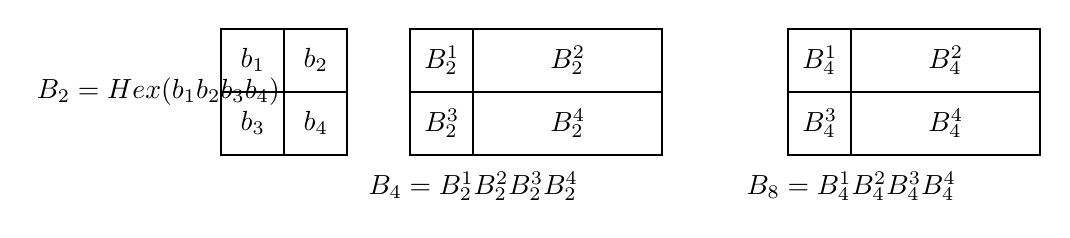
\begin{tikzpicture}[scale=0.8]
        % Draw the first grid
        \draw[thick] (0,0) rectangle (2,2);
        \draw[thick] (0,1) -- (2,1);
        \draw[thick] (1,0) -- (1,2);
        \node at (0.5, 1.5) {$b_1$};
        \node at (1.5, 1.5) {$b_2$};
        \node at (0.5, 0.5) {$b_3$};
        \node at (1.5, 0.5) {$b_4$};
        
        % Add the label for B_2
        \node at (-1, 1) {$B_2 = \text{Hex}(b_1 b_2 b_3 b_4)$};
        
        % Draw the second grid
        \draw[thick] (3,0) rectangle (7,2);
        \draw[thick] (3,1) -- (7,1);
        \draw[thick] (4,0) -- (4,2);
        \node at (3.5, 1.5) {$B_2^1$};
        \node at (5.5, 1.5) {$B_2^2$};
        \node at (3.5, 0.5) {$B_2^3$};
        \node at (5.5, 0.5) {$B_2^4$};
        
        % Add the label for B_4
        \node at (4, -0.5) {$B_4 = B_2^1 B_2^2 B_2^3 B_2^4$};
        
        % Draw the third grid
        \draw[thick] (9,0) rectangle (13,2);
        \draw[thick] (9,1) -- (13,1);
        \draw[thick] (10,0) -- (10,2);
        \node at (9.5, 1.5) {$B_4^1$};
        \node at (11.5, 1.5) {$B_4^2$};
        \node at (9.5, 0.5) {$B_4^3$};
        \node at (11.5, 0.5) {$B_4^4$};
        
        % Add the label for B_8
        \node at (10, -0.5) {$B_8 = B_4^1 B_4^2 B_4^3 B_4^4$};
    \end{tikzpicture}
\end{figure}

The bits ($b_i$) or blocks $B_n^i$ are read in a raster scan order; here $n$ indicates the patch size and $i$, the bit or the block.

\end{document}